\documentclass{vldb}
\usepackage{graphicx}
\usepackage{balance} 
\usepackage{url}
\usepackage{graphicx}

\begin{document}

\title{Providing better confidentiality and authentication on the Internet using Namecoin and MinimaLT}

\numberofauthors{1}
\author{
\alignauthor
Frederic Jacobs\\
\affaddr{www.fredericjacobs.com}\\
\email{me@fredericjacobs.com}
}

\maketitle

\begin{abstract}
In this paper, we introduce a duo of improvements for the Internet that would lead to better security. The authentication model on the Internet is broken and TLS connections have a considerable overhead. We try to address those issues with changes at both the application layer, introducing a replacement for the DNS system, and at the transport layer, a drop-in replacement for TCP built on top of UDP that requires no changes at the network layer.
\end{abstract}

\section{Introduction}

\subsection{Defining user privacy}
The solutions brought forward in this paper are attempts to fix confidentiality and authentication on the Internet. Anonymity is not provided. An attacker could still get a significant amount of metadata. Unfortunately, because MinimaLT runs over UDP you can't connect through the Tor network.\footnote{If MinimaLT proves to be a safer and faster alternative to TLS, I imagine that the Tor project would look into implementing it to speed up the network and make relay connections safer.}
\subsection{Motivation}

When the Internet was designed at DARPA, the primary goal was to design a system that could provide interconnection between multiple computers. The Web then came by with the motivation to be able to freely exchange information. The Internet has mainly been used for open communications. Any computer on the network could request files. But, over time, people started trusting the internet more and more and with the appearance of services. But the Internet grew so quickly out of what DARPA proposed for a trusted environment. The Internet was never designed to be ran by so many different entities and the threat model implied that you had to trust the entities running the infrastructure of the internet.

\section{Domain names and authenticity}

In today's model, if I want to load a page from \emph{facebook.com}, my computer will have to first get the Domain Name System records matching that domain. DNS was designed in a hierarchical way and TLD registrations are handled by a single organisation, the ICANN.

So what is wrong with DNS?

When the original Domain Name System was designed, it did not include security; instead it was designed to be a scalable distributed system. The DNSSEC attempted to add security, while maintaining backwards compatibility. Those security extensions added public key signing to DNS zones but who is signing those zones? The DNS Root Zone, of course. You will then have to trust those too. We thus consider DNSSec as an attempt to try to fix a broken system. We want to design a distributed system where anyone can register a domain but without having a central registration authority.

But how can we verify authenticity? 
Even if my domain name system returns the right IP address how do I know for sure that I'm establishing a connection with the client I want. Today, we are using another hierarchical system to verify authenticity, namely SSL certificates. This means that in addition to trusting ICANN, we will have to trust hundreds of Root Certificate Authorities that are shipped with out browsers.\cite{mozillaSSL}

If only one of those 100s of CA gets compromised, it could result in the man-in-the-middling of any user without any warning since a root certification authority can generate a fake valid certificate for any website. This is what happened in Iran after the Dutch certificate authority DigiNotar got compromised\cite{diginotarHack}.

Now that we are convinced that the hierarchical trust model of the internet is broken, what measures have already been taken to fix authentication on the Internet?

\subsubsection{Certificate Pinning}

The Chrome Security team, led by Adam Langley led the way by implementing certificate pinning. Certificate pinning is a reasonably effective measure for a centralised internet, where only a few websites gather most of the traffic. Certificate pinning works by shipping \emph{pins} in the browser's binary.\cite{chromiumPins} Every time a user loads a pinned website, the certificate fingerprint is compared to the one provided in the binary. If the signature matches, the client continues the SSL handshake. Otherwise, an error message is shown to the user explaining a secured connection couldn't be established.

Although this is a very efficient method to verify SSL certificates, this method doesn't scale and is hard to maintain at a larger scale. In addition to that, the Chromium team needs to verify the "pin" definition before merging every pin request into the code branch. Therefore only larger websites do have certificate pins.

\subsubsection{TACK}

TACK is a proposal by Moxie Marlinkspike and Trevor Perrin, it's a way to 'pin' TLS servers to the correct public key even when a Certificate Authority is telling you differently. Although this is a promising proposition, it doesn't protect against an attacker that has a long-term MITM capability since pins are set on the first connections and do expire after some time.\cite{tackMITM}

\subsubsection{DANE}

The IETF proposal called \emph{DANE} is an attempt at making large scale certificate pinning but by distributing the certificate fingerprint by DNS. This would enable website owners to specify their certificate fingerprint as a DNS entry and visitors would thus be able to verify the authenticity of the server.

Even if we consider that DNSSec does provide good security, this system does still rely on the trust on ICANN and will thus not match the security we want to achieve.

\subsubsection{Tor Hidden Services}

Tor hidden services are reachable by hashes of public keys. This is of course the ideal case when it comes to security because the address contains itself information about the key itself. Unfortunately, humans are not good at remembering pseudorandom 16-character long strings.

\subsection{Zooko's triangle}
In this section, we are introducing Zooko's triangle conjecture and our attempt to square it.

\begin{figure}[h!]
\centering
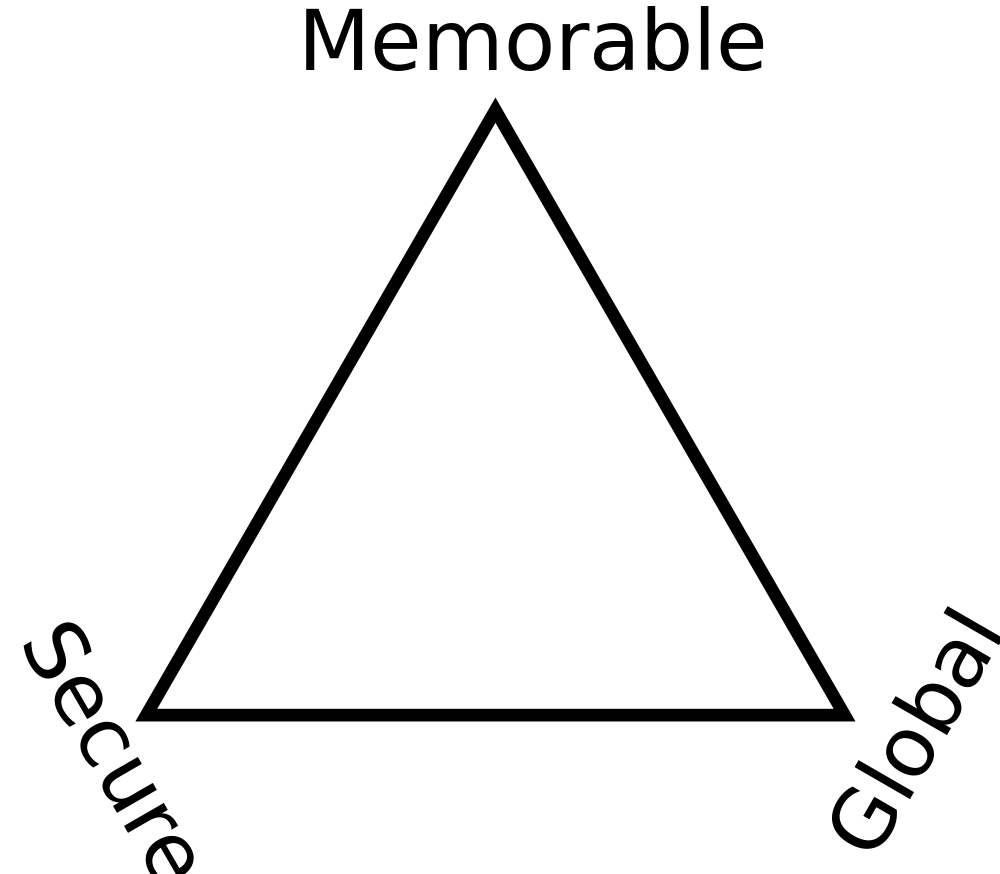
\includegraphics[width=0.3\textwidth]{ZookoTriangle.png}
\end{figure}

Zooko's triangle says that out of these three properties \cite{zookoTriangleWikipedia}, you can usually take only two.
\begin{itemize}
\item \emph{Secure}\footnote{We can't agree with the naming of this property given the threat model we described previously in this paper.}: The quality that there is one, unique and specific entity to which the name maps.
\item \emph{Global}: The lack of a centralized authority for determining the meaning of a name. Instead, measures such as a Web of trust are used.
\item \emph{Memorable}: The quality of meaningfulness and memorability to the users of the naming system.
\end{itemize}

We can thus see that the systems proposed so far only gather two out of three of those properties. If we take the DNS(Sec) system with DANE extensions, we can have a memorable address that is "secure" but unfortunately doesn't have the global property because the ICANN is a centralized authority. Alternatively, Tor's Onion addresses do have the "secure" property and are global but a 16 character pseudorandom string is not memorable.

\subsection{Squaring Zooko's Triangle}

In the following section we are introducing a naming system that is an attempt at squaring Zooko's triangle.

Back in January 2011, Aaron Swartz described on his blog about how Bitcoin blockchain could help in squaring Zooko's triangle. A few months later, a first implementation of that idea came into existence, Namecoin.

\subsubsection{The Bitcoin Blockchain}

The blockchain is Bitcoin's main innovation. Blockchains are data-structures that were invented specifically for the Bitcoin project but they can be applied anywhere a distributed consensus needs to be established in the presence of malicious or untrustworthy actors.

Let's say Alice wants to send money to Bob. Bitcoin addresses are hash
\begin{center}
Key-Hash = RIPEMD-160(SHA-256(public key))
$\text{BTC}_{\text{Address}}$ = Base58(Version +\footnote{The + sign is a string concatenation} Key-Hash + Checksum)
\end{center}
In Bitcoin, the blockchain is used to log all of the transactions. But how does the blockchain work? What prevents anyone to append malicious entries at the bottom of the blockchain.



\subsubsection{Proof of work}

The concept of \emph{proof of work} is used to merge the blockchain. It makes adding entries in the blockchain an expensive process computationally wise. Let's say Alice wants to send Bitcoins to Bob. Alice will start gossiping on the network, telling everyone she wants to send money to Bob. Every client, has a copy of the blockchain and can thus assess if Alice has the amount of money she wants to transfer to Bob. If she has so, gossip will spread. 

Let's say Alice wants to register a domain name name. To achieve that, Alice needs money. The currency used in our model to buy domain names is called the Namecoin. Alice can exchange USDollars or Bitcoins to get those Namecoins. 

Just like Bitcoin, Namecoin is a crypto-currency but in addition to being a cryptocurrency, Namecoin doubles as being a decentralized key-value store.


\subsection{Known Issues with this new model}

\section{Transport security}
What's wrong with tcp is slow and insecure. How to move away from it? Well, we don't really have any other option to base it on UDP.
But we love reliability!

Minimalt  

Multipath TCP advantage?

Doesn't solve anonymity ==> Tor

Issues with too big frames for firewalls?
\section{The {\secit Body} of The Paper}


\section{Conclusions}

% ensure same length columns on last page (might need two sub-sequent latex runs)
//\balance

%ACKNOWLEDGMENTS are optional
\section{Acknowledgments}
Most of the Namecoin research is based on Greg Slepak's work.
\bibliographystyle{abbrv}
\bibliography{bibliography}
\subsection{References}

\begin{appendix}
Define Perfect forward secrecy

Using Elliptic curve crypto but not backdoored.

Impact on censorship( when encrypted blobs can be transferred)
\section{Final Thoughts}

\end{appendix}

\end{document}
